\documentclass[12pt]{article}
\usepackage[left=2cm,top=2cm,right=2cm,bottom=2cm]{geometry}
\usepackage[parfill]{parskip}
\usepackage{amsmath}
\usepackage{graphicx}
\usepackage{listings}
\lstloadlanguages{python}
\usepackage{amssymb}
\usepackage{braket}
\usepackage{pdfpages}
\usepackage{hyperref}
\usepackage{cleveref}
\usepackage{float}
\usepackage{physics}
%\usepackage{minted}
%\usemintedstyle{pastie}


\begin{document}
    \begin{titlepage}
        \begin{center}
            \vspace*{5cm}
            
            \Huge
            \textbf{Milestone 1}
            
            \vspace*{0.5cm}
            \LARGE
            AST5220
        
            \vspace*{0.5cm}
        
            \textbf{Julie Thingwall}
        \end{center}
    \end{titlepage}

\section{Introduction}
    In this projet we wish to follow in the footsteps of Petter Callin\cite{callin2006calculate} who numerically reproduces the power spectrum obtained by the CMB data. This will be done in several steps, where each step simulates the different physical processes that make up the power spectrum.
    
    The first step is to model the background cosmology, how the universe and its contents evolve in time without any perturbations. Specifically, we will explore how the Hubble parameter and the different relative density components of the universe evolves in time. We will also solve the ODE describing how the conformal time behaves. This will be done by utilizing the \textit{very impressive and user friendly} C++ code base provided by our lecturer Hans Winther.



\section{Theory}
\subsection{The Friedman equation and density components}
General relativity tells us, in short terms, that if put stuff with matter or energy in space, then space will change, bend and behave interesting, depending on the nature of the stuff we put in. Using GR, it is possible to obtain expressions that describes how space behaves, given its stuff! 

One such expression is the first Friedman equation. It tells us how the universe as a whole evolves in time, given some density components. It reads as 

\begin{equation}\label{eq:Friedmann Equation}
    H = H_0\sqrt{\left(\Omega_{b,0} + \Omega_{CDM,0}\right)a^{-3} + \left(\Omega_{\nu,0} + \Omega_{r,0}\right) a^{-4} + \Omega_{k,0} a^{-2} + \Omega_{\Lambda,0}},
\end{equation}

where $H=\frac{\dot{a}}{a}$ is the Hubble parameter, $H_0$ is the Hubble parameter today, and the $\Omega_{x}$s are the different relative density components of the universe, namely baryons, cold dark matter, neutrinos, radiation, curvature and dark energy respectively. The 0-subscripts means the value of the relative densities today.  $a(t)$ is the scale factor, which measures the size of the universe relative to today. Further on, we will assume a spatially flat universe with no neutrinos, such that $\Omega_k = \Omega_{\nu} = 0$.

In general, the relative densities are defined as 

\begin{equation}\label{eq:omega def}
    \Omega_x = \frac{\rho_x}{\rho_c}
\end{equation}

where $\rho_x$ is the density of that given component, and $\rho_c = \frac{3H}{8\pi G}$ is the critical density. 

How the $\rho_x$ in \cref{eq:omega def} evolves in time is governed by the continuity equation 

\begin{equation}
    \dot{\rho} + 3H\rho(1 + \omega) = 0
\end{equation}

where $\omega = \frac{P}{\rho}$ is the equation of state. Solving this equation with respect to $a$ yields 
\begin{equation}\label{eq:density time evolution}
\rho = \rho_0 a^{-3(1+\omega)}.
\end{equation}

For matter (baryons and dark matter), $\omega = 0$. For radioation, it is $\omega = 1/3$ and for dark energy, it is $\omega = 0$. 

Inserting \cref{eq:density time evolution} into \cref{eq:omega def} for each component, and doing some mathemagics, we end up with the four equations defined in \cref{eq:Density parameters}. This set of equations governs how each component evolves in time. 

\begin{align}\label{eq:Density parameters}
    \begin{split}
    \Omega_b(a) &= \frac{\Omega_{k,0}}{a^3 H^2/H_0^2}  \\
    \Omega_{CDM}(a) &= \frac{\Omega_{CDM,0}}{a^3 H^2/H_0^2}  \\
    \Omega_r(a) &= \frac{\Omega_{k,0}}{a^4 H^2/H_0^2}  \\
    \Omega_{\Lambda}(a) &= \frac{\Omega_{k,0}}{H^2/H_0^2} 
    \end{split}
\end{align}

Here, $\Omega_{r,0}$ is calculated using the temperature of the CMB today ($T_{cmb}$) by the following formula: 
\begin{equation}
    \Omega_{r,0} = 2 \cdot \frac{\pi^{2}}{30} \frac{\left(k_{b} T_{\mathrm{CMB}}\right)^{4}}{\hbar^{3} c^{5}} \cdot \frac{8 \pi G}{3 H_{0}^{2}}
\end{equation}

\subsection{Conformal Time}
As the universe is strictly growing, size and time are strongly connected. The smaller the universe, the younger it is. This means we can use different quantities describing both lengths and time as our time variable. One of these quantities is the scale factor $a(t)$, but we can also define another variable, namely the conformal time:
\begin{equation}\label{eq:Conformal time integral}
    \eta(a) = \int_0^a \frac{c}{a\mathcal{H}}\textrm{d}a,
\end{equation}

or on ODE form

\begin{equation}\label{eq:conformal time ode da}
    \frac{d\eta}{da} = \frac{c}{a\mathcal{H}}.
\end{equation}

The conformal time is defined as the distance a photon has traveled since the big bang where $t=0$. Here, we also introduce the useful notation $\mathcal{H} = aH$. 


\section{Method and implementation}
\subsection{Code structure}
For the first milestone, all implementations where done in the \texttt{BackgroundCosmology.cpp}. The ODEsolver funciton and Spline function utilizes tools from GSL. All visualisation were done using Python, and can be found in the file \texttt{milestone1\_plots.py}.

\subsection{Time variable}
As we're looking at a timescale ranging over several orders of magnitude, we introduce the logarithmic time scale $x = \ln{a}$. We're specifically interested in the range $a\in [10^{-7},1]$, or $x \in [-16,0]$. This means we subsituted $a = e^x$ in all relevant equations. 

In order to avoid errors or weird behaviour in the end points when splining the $\eta$ function, we solved all equations in the range $x \in [-20,5]$ and then disregarded the points outside $x \in [-16,2]$ in the analysis. We looked at $x_{max} = 2$ instead of $0$ simply because the dark energy dominated era ended up being very close to $x=0$, so extending the range a bit made it easier to see all three eras clearly in the plots. 

\subsection{Cosmological parameters}
All solutions were opbtained using the following cosmological parameters: 
\begin{align*}
    \Omega_{b,0} &= 0.046\\
    \Omega_{CDM,0} &= 0.224\\
    \Omega_{r,0} &= 5.04318\times 10^{-5}\\
    \Omega_{\Lambda,0} &= 0.72995 \\
    h &= 0.7 \\
    T_{cmb} &= 2.725
\end{align*}

\subsection{Obtaining solutions}
We started with implementing the Friedman equation (\cref{eq:Friedmann Equation}) and the relative densities (\cref{eq:density time evolution}) into the code base. This was pretty straight forward. The time evolution of all densities where plotted in the same figure. To make sure everything was implemented correctly, we also plotted the sum of all densities, which should be $1$ at all times. 

To emphasize the three different eras of the universe, namely the radiation dominated, matter dominated and dark matter dominated era, we found the $x-values$ where $\Omega_r = (\Omega_b + \Omega_{CDM})$ and $(\Omega_b + \Omega_{CDM}) = \Omega_{\Lambda}$. This was also added in the plot, represented by three different background colors.

Further on, we solved the differential equation \cref{eq:conformal time ode da}. To do this, we first had to rewrite it as a differential equation with respect to $x$, not $a$. 
\begin{align}\label{eq:conformal time ode dx}
    \frac{d\eta}{da} &= \frac{d\eta}{dx}\frac{dx}{da} = \frac{d\eta}{dx}\frac{1}{a} \nonumber \\ 
    \frac{d\eta}{dx} &= \frac{c}{\mathcal{H}}
\end{align}

\cref{eq:conformal time ode dx} was solved using the ODEsolver from the code base, and the results were promptly splined with the Spline function provided. For initial conditions, we simply assume that $\eta(x=-20) = 0$, meaning a particle horizon of size $0$ when the scale factor is $a=e^{-20}$, which seems sufficiently reasonable!

The results for $\eta(x)$ where plotted next to $H(x)$, $H(z)$ and $\mathcal{H}(x)$. As with the relative densities, we indicate the different eras with different background colors.

\section{Results}
In \cref{fig:omega} we see the time evolution for all relative densities. The different eras are clearly visible even when not considering the background colors. We first see that radiation dominates the early universe (yellow) up until matter-radiation equality at $x=-8.57$ or $z\approx 5000$, where we enter the matter dominated era (blue) until we reach matter-dark energy equality at $x=-0.32$, or $z\approx 0.38$, where the dark energy dominated era begins. 

The red stippled line is the sum of all $\Omega_i$ at all times, which we can see is always promptly at $1$, as it should be! But as any good cosmologist should know, radiation/matter equality happened at around $z\approx 3600$, so we're a bit off the mark here? 

In \cref{fig:H_eta} we see how the Hubble parameter, $\mathcal{H}$ and the conformal time evolves in time. The plots for $H(x)$ and $H(z)$ shows how the Hubble parameter decreases at different rates in the radiation and matter dominated eras, while it flattens out as constant in the dark energy dominated era. For $\mathcal{H}$, however, the accelerated expansion caused by dark energy is clearly visible. This makes sense when recalling that the definition for $\mathcal{H} = aH = \dot{a}$. Finally, the lower right plot shows how $\eta(x)$ evolves. It is increasing, but less so for each era.

\begin{figure}[h]
    \centering
    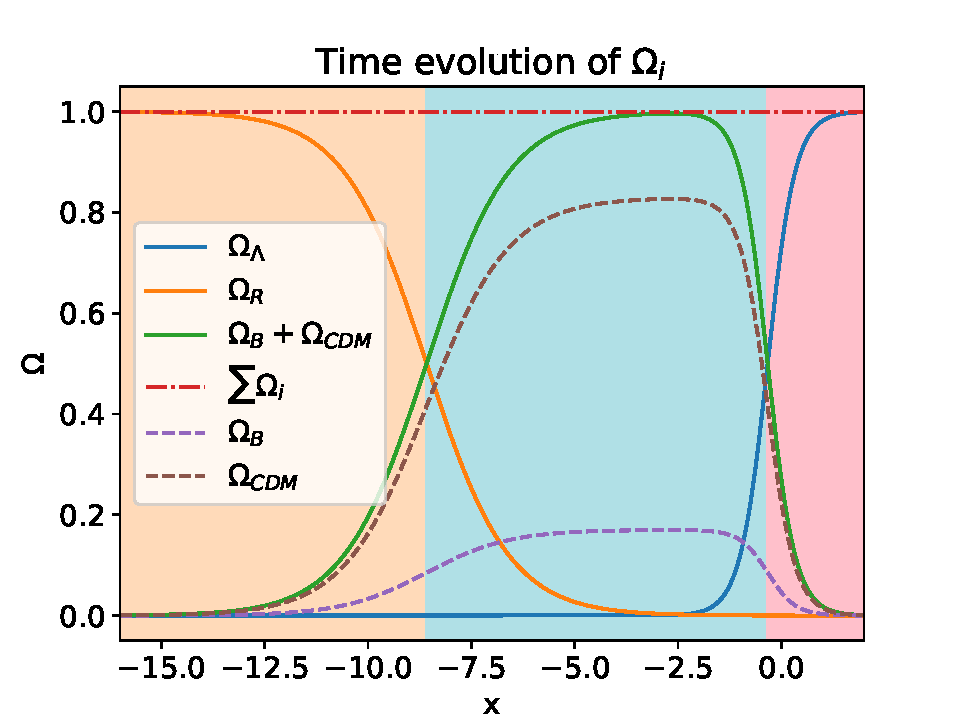
\includegraphics[width=0.9\textwidth]{omega_plot.pdf}
    \caption{Plot showing how the different density parameters evolve as a function of x. The radiation dominated era, matter dominatied era and dark matter dominated era are indicated by the yellow, blue and red background colors respectively.}
    \label{fig:omega}
\end{figure}

\begin{figure}[h]
    \centering
    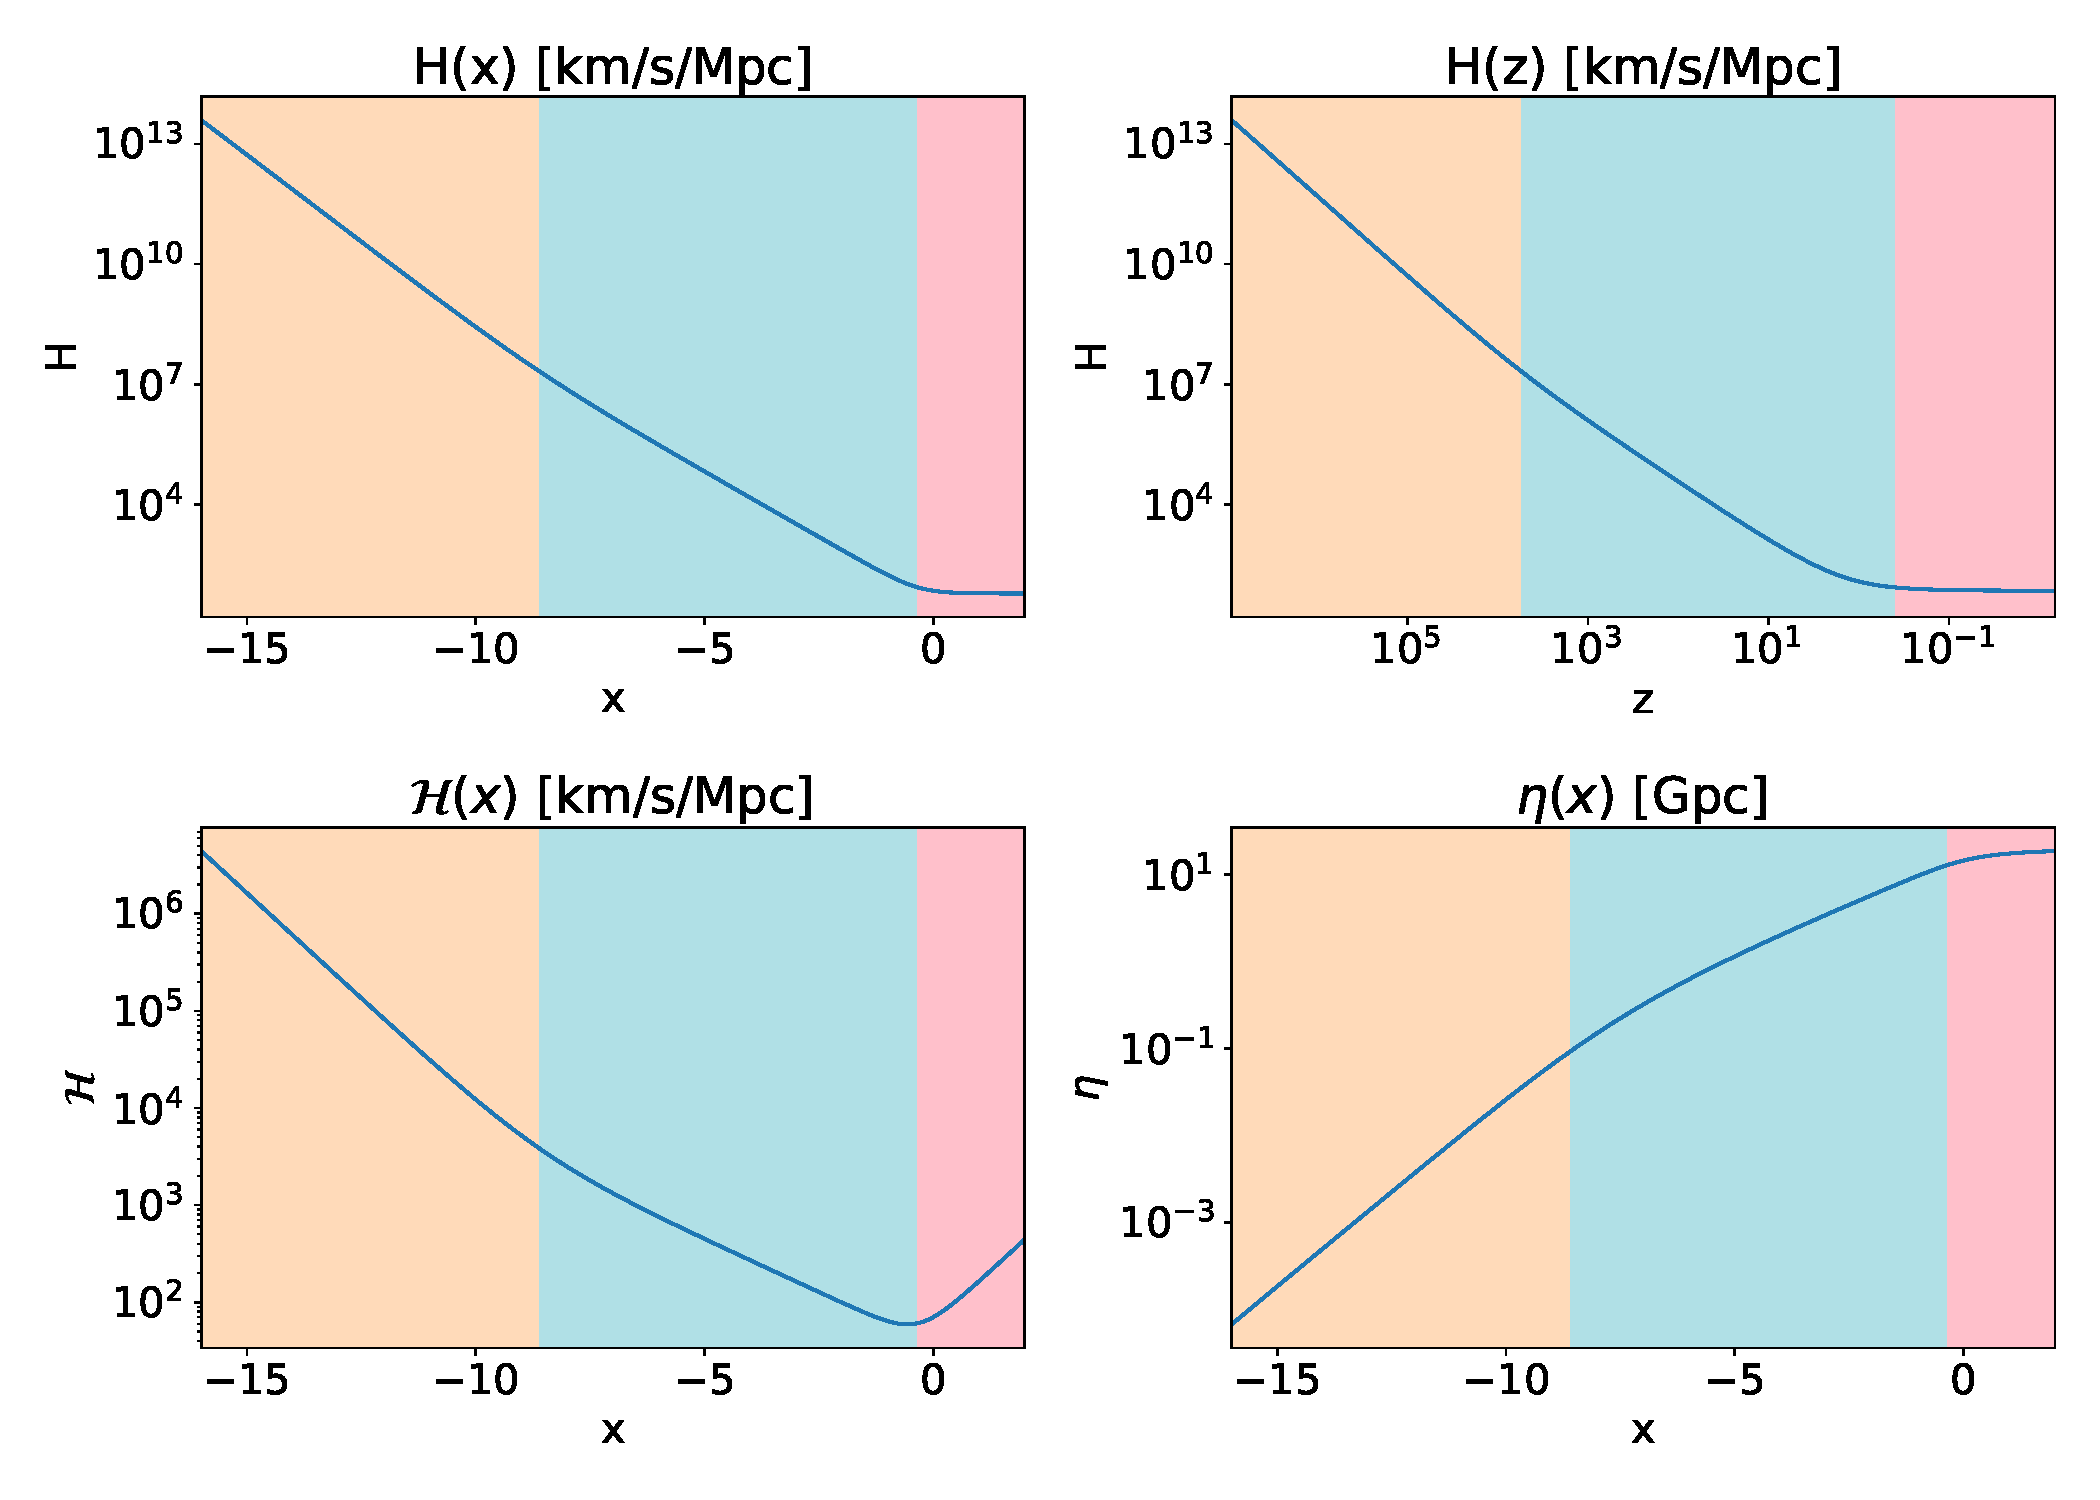
\includegraphics[width=0.95\textwidth]{H_eta_plots.pdf}
    \caption{Plots showing how the Hubble parameter and the conformal time $\eta$ evolves in time. The two upper figures show how the Hubble parameter evolves with respect to $x$ and the cosmological redhist $z$. The lower left picture shows how $\mathcal{H}$ evolves as a function of x. The lower right shows the evolution of $\eta(x)$. As in \cref{fig:omega}, the background colors indicate the different eras of the universe.}
    \label{fig:H_eta}
\end{figure}

\bibliography{bibtex}{}
\bibliographystyle{plain}


\end{document}